\documentclass[12pt, twoside]{article}
\usepackage[letterpaper, margin=1in, headsep=0.5in]{geometry}
\usepackage[english]{babel}
\usepackage[utf8]{inputenc}
\usepackage{amsmath}
\usepackage{amsfonts}
\usepackage{amssymb}
\usepackage{tikz}
\usetikzlibrary{quotes, angles}
\usepackage{graphicx}
\usepackage{enumitem}
\usepackage{multicol}

\newif\ifmeta
\metatrue %print standards and topics tags

\title{Regents Geometry}
\author{Chris Huson}
\date{September 2020}

\usepackage{fancyhdr}
\pagestyle{fancy}
\fancyhf{}
\renewcommand{\headrulewidth}{0pt} % disable the underline of the header
\raggedbottom


\fancyhead[LE]{\thepage}
\fancyhead[RO]{\thepage \\ Name: \hspace{4cm} \,\\}
\fancyhead[LO]{BECA / Dr. Huson / Geometry 01-Intro\\* pset ID: 0}

\begin{document}

\subsubsection*{1-1CW-Measurement}
\begin{enumerate}
\item Given the line segment $\overline{PQ}$ shown below. Answer the questions and complete as directed.
    \begin{enumerate}
      \item Measure the length of the segment in centimeters. $PQ=$
      \bigskip
      \item Is the segment horizontal, vertical, or diagonal?
      \bigskip
      \item With a compass, draw a circle centered at $P$ that passes through $Q$.
      \bigskip
      \item Draw a circle centered at $Q$ that passes through $P$.
    \end{enumerate}
    \vspace{7cm}
    \begin{center}
    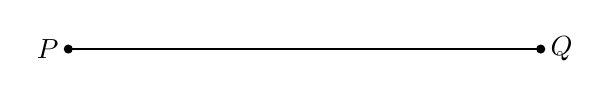
\begin{tikzpicture}
      \draw [-, thick] (0,0)--(6,0);
      \draw [fill] (0,0) circle [radius=0.05] node[left]{$P$};
      \draw [fill] (6,0) circle [radius=0.05] node[right]{$Q$};
    \end{tikzpicture}
    \end{center}
  
\newpage

\item Given an angle with vertex $A$. Answer the questions and complete as directed.
    \begin{enumerate}
      \item Using a compass, measure angle $A$ in degrees. $m\angle A =$
      \bigskip
      \item Mark and label a point $B$ that is 4 centimeters from $A$ on the horizontal ray.
      \bigskip
      \item Draw a circle centered at $A$ with a radius of 4 centimeters. \bigskip
    \end{enumerate}
    \vspace{3cm}
    \begin{center}
    \begin{tikzpicture}
      \draw [<->, thick] (45:9)--(0,0)--(9,0);
      \draw [fill] (0,0) circle [radius=0.05] node[below]{$A$};
      %\draw [fill] (7,0) circle [radius=0.05] node[below]{$N$};
    \end{tikzpicture}
    \end{center}

\newpage
\item Given the rectangle $ABCD$ shown below. Answer the questions and complete as directed.
    \begin{enumerate}
      \item Measure the length of the rectangle in centimeters. $AB=$
      \bigskip
      \item Measure the height of the rectangle in centimeters. $AD=$
      \bigskip
      \item Calculate the area of the rectangle in square centimeters.
      \vspace{2cm}
      \item Using a straight edge, draw a diagonal from point $A$ to $C$.
      \bigskip
      \item Lightly shade the bottom triangle, $\triangle ABC$.
      \bigskip
      \item Of the two triangles, $\triangle ABC$ and $\triangle CDA$, which has a larger area, or are they the same?
      \vspace{2cm}
      \item Measure the length of the diagonal. $AC=$
    \end{enumerate}
    \vspace{2cm}
    \begin{center}
    \begin{tikzpicture}
      \draw [-, thick] (0,0)--(11,0)--(11,5)--(0,5)--cycle;
      \draw [fill] (0,0) circle [radius=0.05] node[below]{$A$};
      \draw [fill] (11,0) circle [radius=0.05] node[below]{$B$};
      \draw [fill] (11,5) circle [radius=0.05] node[right]{$C$};
      \draw [fill] (0,5) circle [radius=0.05] node[left]{$D$};
    \end{tikzpicture}
    \end{center}

\newpage
\item The points shown are in a straight line, $\overline{ABC}$. Given the lengths $AB=4$ cm and $BC=2$ cm.
  \begin{enumerate}
    \item Calculate the length ${AC}$.\\[1.5cm]
      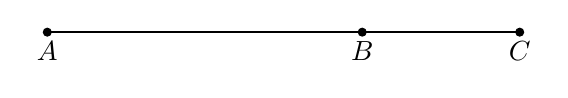
\begin{tikzpicture}
        \draw [-, thick] (1,0)--(7,0);
        \draw [fill] (1,0) circle [radius=0.05] node[below]{$A$};
        \draw [fill] (5,0) circle [radius=0.05] node[below]{$B$};
        \draw [fill] (7,0) circle [radius=0.05] node[below]{$C$};
      \end{tikzpicture} \vspace{1cm}
    \item Justify your answer.
  \end{enumerate} \vspace{3cm}

\item Given $\overleftrightarrow{QS}$ as shown on the number line. \\[20pt] % Midpoint
    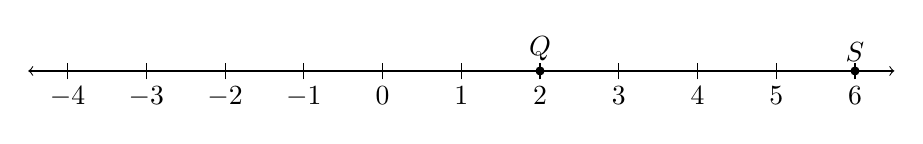
\begin{tikzpicture}
      \draw [<->] (-4.5,0)--(6.5,0);
      \foreach \x in {-4,...,6} %2 leading for diff!=1
        \draw[shift={(\x,0)},color=black] (0pt,-3pt) -- (0pt,3pt) node[below=5pt]  {$\x$};
        \draw [fill] (2,0) circle [radius=0.05] node[above] {$Q$};
        \draw [fill] (6,0) circle [radius=0.05] node[above] {$S$};
    \end{tikzpicture} \bigskip
    \begin{enumerate}
      \item In the given number line units, what is the distance between $Q$ and $S$? $QS=$
      \bigskip
      \item Mark the point $R$, the midpoint of $\overline{QS}$.
    \end{enumerate}\vspace{2cm}

\end{enumerate}
\end{document}